\chapter{Theoretical introduction and motivation}\label{chap:introduction}
\minitoc

In this chapter, at first the relevant unit system is introduced. Afterwards, the standard model of particle physics is explained by discussing its particle content and the interactions between the particles. Thereafter, the important properties and concepts of supersymmetry are outlined, while focusing in particular on gauge-mediated supersymmetry and considered signal scenarios. In the end, a brief overview of the current status of searches for supersymmetry at the LHC is given.



\section{System of units}\label{sec:units}

For simplicity, the unit system commonly used in particle physics is the natural unit system~\cite{UnitSystem}. In natural units, the reduced Planck constant $\hslash$ and the speed of light $c$ are set to unity:
\begin{equation}
 \hslash=c=1.
\end{equation}
The observables used most frequently in particle physics are the energy, the momentum, and the mass. They are given in magnitudes of $\eV$ in the natural unit system. For other variables, such as length and time, the metric unit system is used. Cross sections are given in barn $\left(1\barn=10^{-28}\m^2\right)$. Integrated luminosities are therefore given in $\binv$. Electric charges are given in dependence of the elementary charge $e$.

\section{The standard model of particle physics}\label{sec:SM}

The standard model of particle physics (SM) is a gauge theory describing three of the four fundamental forces, namely the electromagnetic, the weak, and the strong interactions~\cite{SM}. The gravitational force is described by general relativity~\cite{Einstein}, which is not described in a quantum field theory as the other three forces.\\
All particles can be divided into two categories: Particles of integer spin, called bosons, and particles of half-integer spin, called fermions.\\\\
The matter content is given by the fermions. Fermions are divided into two subgroups, called quarks and leptons. Leptons take part only in electroweak interactions, while quarks carry also a color charge and therefore interact via the strong force. There are three generations of fermions, which include each two leptons and two quark flavors. The quark flavors are the down, up, strange, charm, bottom, and top quarks, while the lepton flavors are made up of three electrically charged particles, the electron ($\Pe$), the muon ($\PGm$), and the tau lepton ($\PGt$), as well as three electrically neutral leptons, called neutrinos ($\Pgne,\Pgngm,\Pgngt$).
% The latter are assigned the names of the charged leptons of the same generation.
Of the quarks, there are up-type quarks, the up, charm, and top quark, carrying an electric charge of $+\frac{2}{3}e$, and down-type quarks, the down, strange, and bottom quark, carrying an electric charge of $-\frac{1}{3}e$.\\
The SM is based on the symmetry group $SU(3)\otimes SU(2)\otimes U(1)$. Interactions are described via the exchange of spin-1 gauge bosons. In case of the strong force, these are 8 massless gluons, which carry color charge and couple to it. The mediator of the electromagnetic interaction is the massless photon, coupling to the electric charge of particles. For the weak interaction the responsible mediator particles are the three massive bosons $\PWpm$ and $\PZ$, which couple to the weak isospin.\\\\
An illustration of the complete SM particle content with its properties is shown in \refFig{fig:SM}.
For each particle, a corresponding antiparticle exists with same mass and inversed quantum numbers. Throughout this thesis particles and antiparticles are treated the same way, and both are labeled with the name of the particle.\\

\begin{figure}[tbp]
 \centering
 \includegraphics[width=0.8\textwidth]{figures/general/SM}
 \caption{Complete particle content of the standard model~\cite{SMPlot}. For each particle important properties such as mass, spin, and charges are given. The values are taken from~\cite{PDG}.}
 \label{fig:SM}
 
\end{figure}


The strong interaction between color charged particles is described by the quantum field theory of quantum chromodynamics (QCD). The corresponding mediators of the non-abelian gauge group $SU(3)_C$ are the eight gluons, which carry each the color-charge $C$ of an anticolor and a color, giving rise to the self-coupling of gluons. Due to the confinement of quarks~\cite{Confinement}, quark-antiquark pairs will be produced out of the vacuum if particles with color charge are being separated, since the potential energy density of the strong force includes constant terms, and the potential energy rises with increasing distance. This principle is responsible for the existence of only color-neutral bound states of two (mesons) or three (baryons) quarks, called hadrons. Indications for hadrons made up of five quarks (pentaquarks) have also been found recently~\cite{Pentaquarks}.\\
Based on the same principle, color charged particles are not observed as single particles. In the hadronization process, gluons and quarks lead to the generation of large aggregations of color charged particles while transversing the detector material. These clusters are called jets.
\\\\
The electromagnetic and weak forces are unified in the electroweak theory~\cite{Weinberg,Weinberg2,Salam,Glashow}, represented by the gauge group $ SU(2)_L\otimes U(1)_Y$. The indices $L$ and $Y$ indicate the symmetry of the $U(1)_Y$ group corresponding to the weak hypercharge $Y$, and that the weak isospin $T$ couples only to left-handed $SU(2)_L$ doublets of fermions, while the right-handed $SU(2)_L$ singlets carry no isospin. The three mediators of the $SU(2)_L$ group are the $W^1,W^2$, and $W^3$ bosons, and the gauge boson of the $U(1)_Y$ group is the $B^0$ boson.
% Due to the spontaneous symmetry breaking in the electroweak unification, these four bosons mix to the observed $\PWpm$ and $\PZ$ bosons and the photon $\PGg$:
These four bosons mix to the $\PWpm$ and $\PZ$ bosons and the photon $\PGg$:
\begin{equation}
 \left(
 \begin{matrix}
  \PGg \\
  \PZ
 \end{matrix}
 \right)
 =
 \left(\begin{matrix}
  \cos(\theta_W)  & \sin(\theta_W) \\
  -\sin(\theta_W) & \cos(\theta_W) 
 \end{matrix}\right)
 \cdot
 \left(
 \begin{matrix}
  B \\
  W^3
 \end{matrix}
 \right),
\end{equation}

\begin{equation}
 \PWpm = \frac{1}{\sqrt{2}}\left(W^1\mp i W^2\right),
\end{equation}
where $\sin^2(\theta_W)\approx0.231$~\cite{PDG} is the weak-mixing angle, also referred to as Weinberg angle.
The resulting weak interaction is parity violating~\cite{Wu,Goldhaber}. The $\PWpm$ bosons only couple to left-handed fermions, while the neutral Z boson couples to both left-handed and right-handed particles, but with different strength.\\
\\In this theory, the gauge bosons are not allowed to have dirac mass terms in the Lagrangian, because it would the break local gauge symmetry. However, since the $\PZ$ boson mass is measured to be $91.2\GeV$~\cite{PDG}, and the $\PW$ boson mass to be $80.4\GeV$~\cite{PDG}, the Higgs mechanism is introduced~\cite{Higgs1,Higgs2,Higgs3}. In its simplest representation, it predicts a complex scalar Higgs doublet with a potential that is symmetric, but has a non zero vacuum expectation value. Therefore, the deviation from zero is responsible for the spontaneous symmetry breaking of the $ SU(2)_L\otimes U(1)_Y$ gauge group. The Higgs field can be represented by the complex scalar $SU(2)_L$ doublet
\begin{equation}
 \Phi=
 \left(\begin{matrix}
   \Phi^{+} \\
   \Phi^0
  \end{matrix}
 \right)
 =
 \frac{1}{\sqrt{2}}
 \left(\begin{matrix}
   \Phi_1 + i \Phi_2 \\
   \Phi_3 + i\Phi_4
  \end{matrix}
 \right)
\end{equation}
with the potential
\begin{equation}
 V(\Phi)=\mu^2 \Phi^{\dagger}\Phi+\lambda\left(\Phi^{\dagger}\Phi\right)^2.
\end{equation}
For $\mu^2<0$, it results in the non-zero vacuum expectation value of
\begin{equation}
 v = \frac{|\mu|}{\sqrt{\lambda}}.
\end{equation}
The field can be reformulated without loss of generality by expanding around the vacuum expectation value and transforming to unitary gauge as
\begin{equation}
 \Phi = \frac{1}{\sqrt{2}}
 \left(\begin{matrix}
   0 \\
   v+h
  \end{matrix}
 \right),
\end{equation}
where $h$ is a scalar field. Thereby, three of the four degrees of freedom of the field are consumed to give mass terms to the $\PW$ and $\PZ$ bosons. The remaining degree of freedom is the spin-0 Higgs boson. For consistency, leptons and quarks acquire also masses in the SM via Yukawa interactions with the Higgs field.
Such a neutral boson has been observed in proton-proton collisions at the LHC in 2012~\cite{HiggsCMS,HiggsATLAS}, and its mass has been determined to be $125.09\pm0.24\GeV$. Measurements regarding the Higgs boson are in good agreement with SM predictions~\cite{HiggsPrecise}, and recently also the couplings of Higgs bosons to the top quark~\cite{ttH}, and decays of Higgs bosons to bottom quarks and tau leptons have been observed~\cite{HiggsTauTau,HiggsBB}, strengthening the presumption, that the found Higgs boson is the postulated SM Higgs boson.



\subsection*{Indications for physics beyond the standard model}\label{sec:SM_bsm}
Although the SM describes all phenomena observed at high energy particle colliders successfully, different observations and theoretical arguments indicate that there must exist physics beyond the standard model (BSM):
\begin{enumerate}
 \item Precise measurements of the cosmic microwave background and theoretical interpretations suggest, that only $4.9\%$ of the universe consists of ordinary matter, while the remainder is composed of dark energy and dark matter~\cite{DarkMatterPlanck}. The existence of dark matter is also observed in gravitational lensing effects~\cite{DarkMatterLensing} and in the velocity of rotation curves of spiral galaxies~\cite{DarkMatterRotation}. Inside the SM, there exists no particle that could explain the total amount of dark matter in the universe.
 \item It is assumed, that in the early age of the universe there was the same amount of matter and antimatter. But, today we observe the existence of much more matter than antimatter~\cite{Antimatter,AsymSM}. In order to explain this discrepancy, different conditions, such as $\mathcal{CP}$-violation and baryon number violation, must be fulfilled~\cite{Sakharov}. However, in the SM there are no known sources of $\mathcal{CP}$-violation effects large enough to give rise to such big differences, while baryon number conservation is not violated at all.
 \item In the SM, neutrinos are predicted to be massless particles. But, the observation of neutrino oscillations are only explicable if neutrinos are massive particles~\cite{NeutrinoMass,PDG}.
 \item The observation of a Higgs boson in 2012 on the one hand marks the great success of the SM, but on the other hand directly leads to an issue concerning the Higgs mass, which is known as the "Hierarchy Problem". The Higgs boson couples to all massive particles, with coupling strengths proportional to their masses. But unlike for all other particles, the correction to the Higgs boson mass is quadratically divergent at low energies, caused by virtual loop corrections. The cut-off scale for these corrections can be as large as the validity scale of the SM. Thus, the Higgs boson mass can be enlarged to the order of the Planck scale ($10^{19}\GeV$). Since its mass was measured at the LHC to be approximately $125\GeV$, and due to the large difference between the electroweak scale ($10^2\GeV$) and the Planck scale, these correction terms need to cancel extremely precisely over 32 orders of magnitude. This is considered "unnatural", leading to the expectation that new physics exists in the energy range between the electroweak and the Planck scale.
 \item Driven by the electroweak unification, the unification of all forces except for gravity in a grand unified theory (GUT) is well motivated. While the couplings of the forces in the SM do not lead to a unification at very high energies~\cite{PDG}, a possible extension of the SM with additional new particles could realize such a unification of the electroweak and strong interactions, see \refFig{fig:couplings}.
\end{enumerate}
% One of those theories is supersymmetry~\cite{SUSYOriginal}.
\begin{figure}
 \centering
 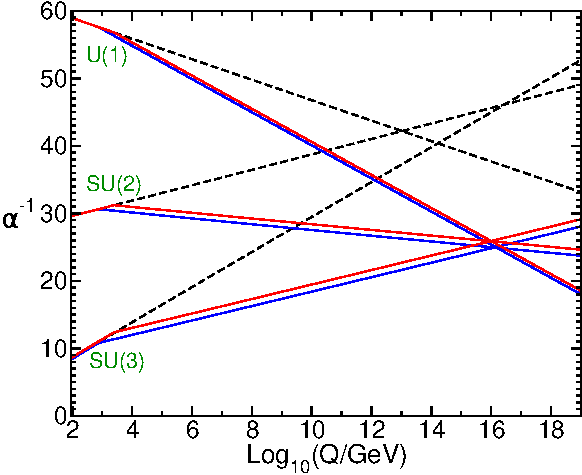
\includegraphics[width=\pairwidth]{figures/general/couplings}
 \caption{Running couplings for all three fundamental forces in case of the SM (dashed lines) and the minimal supersymmetric standard model (solid lines) for two different sparticle mass scales ($750\GeV$ and $2.5\TeV$)~\cite{SUSYPrimer}.}
 \label{fig:couplings}
\end{figure}



\section{Supersymmetry}\label{sec:SUSY}
Supersymmetry (SUSY)~\cite{SUSYOriginal,SUSYPrimer} is one of the most popular BSM theories and was developed in the 1970s~\cite{SUSYTheorem,HAAG1975257}. It is well motivated with regard to the theory, because it is the only possible extension of space time symmetry. Since then, many different SUSY models have been developed, all based on the same principle: SUSY connects fermions with bosons and the other way around by introducing supersymmetric partners for SM particles. These superpartners differ only in spin by $\pm1/2$, and all other quantum numbers are equal. With the help of generators $Q$, bosonic and fermionic states can be transformed into each other:
\begin{equation}
 Q\,\ket{fermion}=\ket{boson},~~~~~~ Q\,\ket{boson}=\ket{fermion}.
\end{equation}
Advantages of SUSY are, \eg, that multiple models directly provide candidates for dark matter particles, it realizes the unification of forces, and solves the Hierarchy Problem without fine tuning of physical parameters to match the observation.\\
The simplest model of SUSY regarding the extension of the particle content is the minimal supersymmetric standard model (MSSM), where only exactly one $Q$ exists. Within the MSSM, for each left and right-handed fermion in the SM exactly one supersymmetric scalar bosons is introduced. To differentiate between SM and SUSY particles, the names of supersymmetric partners are those of the SM particles prepended with an "s-" in case of the fermions. Thus, the partners are called sfermions, and, \eg, the partner of the electron is the selectron. The names of superpartners of bosons are constructed by appending the SM name with an "-ino", making them bosinos, so the gluon's superpartner for example is called gluino. In general, superpartners are called sparticles, and are labeled the same as their SM counterparts, but with a tilde (\eg $\mu \to \widetilde{\mu}$). Also, the couplings between all sparticles are the same as of their SM partners.\\
To realize mass terms in the spontaneous symmetry breaking for all particles, including both up- and down-type fermions, the SM Higgs sector needs to be extended to two complex scalar doublets:
\begin{equation}
 H_u=  \left(
 \begin{matrix}
  H_u^+ \\
  H_u^0
 \end{matrix}
 \right),~~~~~
 H_d=  \left(
 \begin{matrix}
  H_d^0 \\
  H_d^-
 \end{matrix}
 \right).
\end{equation}
The $H_d$ gives masses to the down-type quarks and charged leptons, while the $H_u$ is responsible for the masses of up-type quarks. Four higgsinos as superpartners are introduced in the MSSM accordingly. As a consequence, there are eight degrees of freedom in the Higgs sector instead of four, related to the two Doublets, and giving rise to an expanded Higgs sector consisting of five particles: the two neutral scalars $h^0$ and $H^0$, the two charged scalars $H^{\pm}$, and the neutral pseudoscalar $A^0$. The remaining three degrees of freedom give masses to the gauge bosons as in the SM. The observed Higgs boson at the LHC can be identified as one of the two neutral scalars, where the lightest boson, the $h^0$, is chosen by convention.\\
The gauginos and higgsinos mix, similar to the mixing in the electroweak sector, to eight mass eigenstates, which are the four neutral neutralinos $\neutralinoOne,~\neutralinoTwo,~\neutralinoThree$,~and $\neutralinoFour$, and the four charged charginos $\charginoOne$ and $\charginoTwo$.\\
The total particle content of the MSSM is shown in \refFig{fig:mssm}. To include gravity, the SM is extended by the graviton $G$, and the SUSY sector is extended by its superpartner, the gravitino $\gravitino$.

\begin{figure}[tbp]
 \centering
 \includegraphics[width=0.8\textwidth]{figures/general/MSSM}
 \caption{The particle content of the MSSM extended with the graviton and gravitino. Mixings to mass eigenstates are indicated with the brackets.}
 \label{fig:mssm}
\end{figure}

In unbroken SUSY, the particles and their corresponding sparticles should have the same masses, and those SUSY particles should have been found easily in the past (considering, \eg, a selectron with a mass of $511\keV$). Therefore, SUSY must be a broken symmetry. Many different theories have been developed over time to explain different breaking scenarios. Attractive approaches are models where gravity is responsible for the SUSY breaking~\cite{SUSYPrimer}, anomaly breaking scenarios~\cite{AMSB}, and in particular gauge-mediated supersymmetry breaking, which is discussed in the next section.\\
SUSY can provide Dark Matter candidates, if the lightest supersymmetric particle (LSP) is stable, electrically neutral, and colorless.
R-parity
\begin{equation}
 R = (-1)^{3B+L+S}
\end{equation}
is therefore introduced as a new conserved quantum number, where S is the spin, $B$ the Baryon number, and $L$ the lepton number. The R-parity is $-1$ for sparticles, and $+1$ for particles, respectively.\\
It is not fundamentally necessary that the LSP is stable. In R-parity violating scenarios, decays of all SUSY particles into SM particles are allowed. Hence, the conservation of the Baryon number or the lepton number is violated. R-parity conserving scenarios however are motivated by many precision measurements, such as the lifetime measurement of protons~\cite{ProtonDecay}.
In this thesis, only R-parity conserving scenarios are considered. Therefore, SUSY particles can only be produced in pairs and the LSP needs to be stable.\\



\subsection{General Gauge Mediation}\label{sec:GGM}
The phenomenology of SUSY is very rich. While in many models gravity is responsible for SUSY breaking, a different approach, motivating this search, is general gauge mediation (GGM). It is based on the assumption of gauge mediated supersymmetry breaking (GMSB)~\cite{GGM}, where an additional "hidden sector" is introduced that is responsible for the breaking. This sector is mainly decoupled, and the possible interactions between the visible and the hidden sector are only achieved by messenger fields mediated by gauge interactions. In the studied GMSB models, the LSP is the gravitino $\gravitino$. This particle is assumed to be very light ($\ll1\GeV$). Therefore, the next-to-lightest supersymmetric particle (NLSP), which basically can be any sparticle, decays promptly. Since the gravitino is stable because of R-parity conservation, electrically and color neutral, it will leave the detector undetected, causing an imbalance in the measured total transverse momentum in proton-proton collisions at the LHC.\\
In all models considered throughout this thesis, the NLSP is assumed to be the lightest neutralino ($\neutralinoOne$). In general, the mixing of the NLSP can include bino, wino, and higgsino components, each enabling different decay channels.


\subsection{Signal scenarios}\label{sec:SMS}
The signal scenarios considered in this thesis are discussed in the following. In general, very different production channels for SUSY particles, such as electroweak and strong production, are possible. In case of the LHC proton-proton collisions, SUSY particles can be produced directly in the hard scattering processes of the partons, leading to cascade decays down to the decays of the NLSP to the gravitino and a SM boson. The branching fractions of the lightest neutralino to different SM bosons depends on its mixing
\begin{equation}
 \neutralinoOne = \sum_{i=1}^{N} N_{1i} \widetilde{\psi}_i^0,
\end{equation}
where $\widetilde{\psi}_i^0=(\widetilde{B},\widetilde{W},\widetilde{H}_d^0,\widetilde{H}_u^0)$~\cite{NLSPDecay}. The mass eigenvectors $N_{1i}$ are defined by four parameters, namely the bino mass $M_1$ and the wino mass $M_2$ at the messenger scale, the supersymmetric Higgs mass term $\mu$, and $\tan{\beta}$, the ratio of the up-type to down-type Higgs vacuum expectation values. In GGM, a neutralino NLSP has three possible decay branches, all involving the $\gravitino$~\cite{NLSPDecay}:
% \begin{equation}
\begin{align}
 \Gamma\left(\neutralinoOne\to\gravitino+\PGg\right) & = |N_{11}c_W+N_{12}s_W|^2 \mathcal{A}                                                                                                                       \\
 \Gamma\left(\neutralinoOne\to\gravitino+\PZ\right)  & = \left(|N_{12}c_W - N_{11}s_W|^2 +\frac{1}{2}|N_{13}c_{\beta}-N_{14}s_{\beta}|^2\right)\left(1-\frac{m_{\PZ}^2}{m_{\neutralinoOne}^2}\right)^4 \mathcal{A} \\
 \Gamma\left(\neutralinoOne\to\gravitino+h\right)    & = \frac{1}{2}|N_{13}c_{\beta}+N_{14}s_{\beta}|^2\left(1-\frac{m_{h}^{2}}{m_{\neutralinoOne}^2}\right)^4 \mathcal{A}                                         
\end{align}
% \end{equation}
Here, $c_W$, $s_W$, $c_\beta$, and $s_\beta$ are abbreviations for $\cos(\theta_{\text{W}})$, $\sin(\theta_{\text{W}})$, $\cos(\beta)$, and $\sin(\beta)$, respectively. The formulae hold in cases of on-shell $\PZ$ and $h$ production. $\mathcal{A}$ is a parameter responsible for the NLSP lifetime~\cite{NLSP1,NLSP2}:
\begin{equation}
 \mathcal{A} = \frac{m_{\neutralinoOne}^5}{16\pi F_{0}^{2}}\approx\left(\frac{m_{\neutralinoOne}}{100\GeV}\right)^5\left(\frac{100\TeV}{\sqrt{F_0}}\right)^4 \frac{1}{0.1\mm},
\end{equation}
where $F_0$ is the scale of SUSY breaking, its range is given by $10\TeV\lesssim\sqrt{F_0}\lesssim10^6\TeV$, and it is related to the gravitino mass via
\begin{equation}
 m_{\gravitino}=\frac{F_0}{\sqrt{3}M_{Planck}}.
\end{equation}
% Branching fractions for pure bino- or wino-, or higgsino-like NLSPs are shown in \refFig{fig:BRNLSP}.
Branching fractions for pure bino- or wino-like NLSPs are shown in \refFig{fig:BRNLSP}.
\begin{figure}[htb]
 \centering
 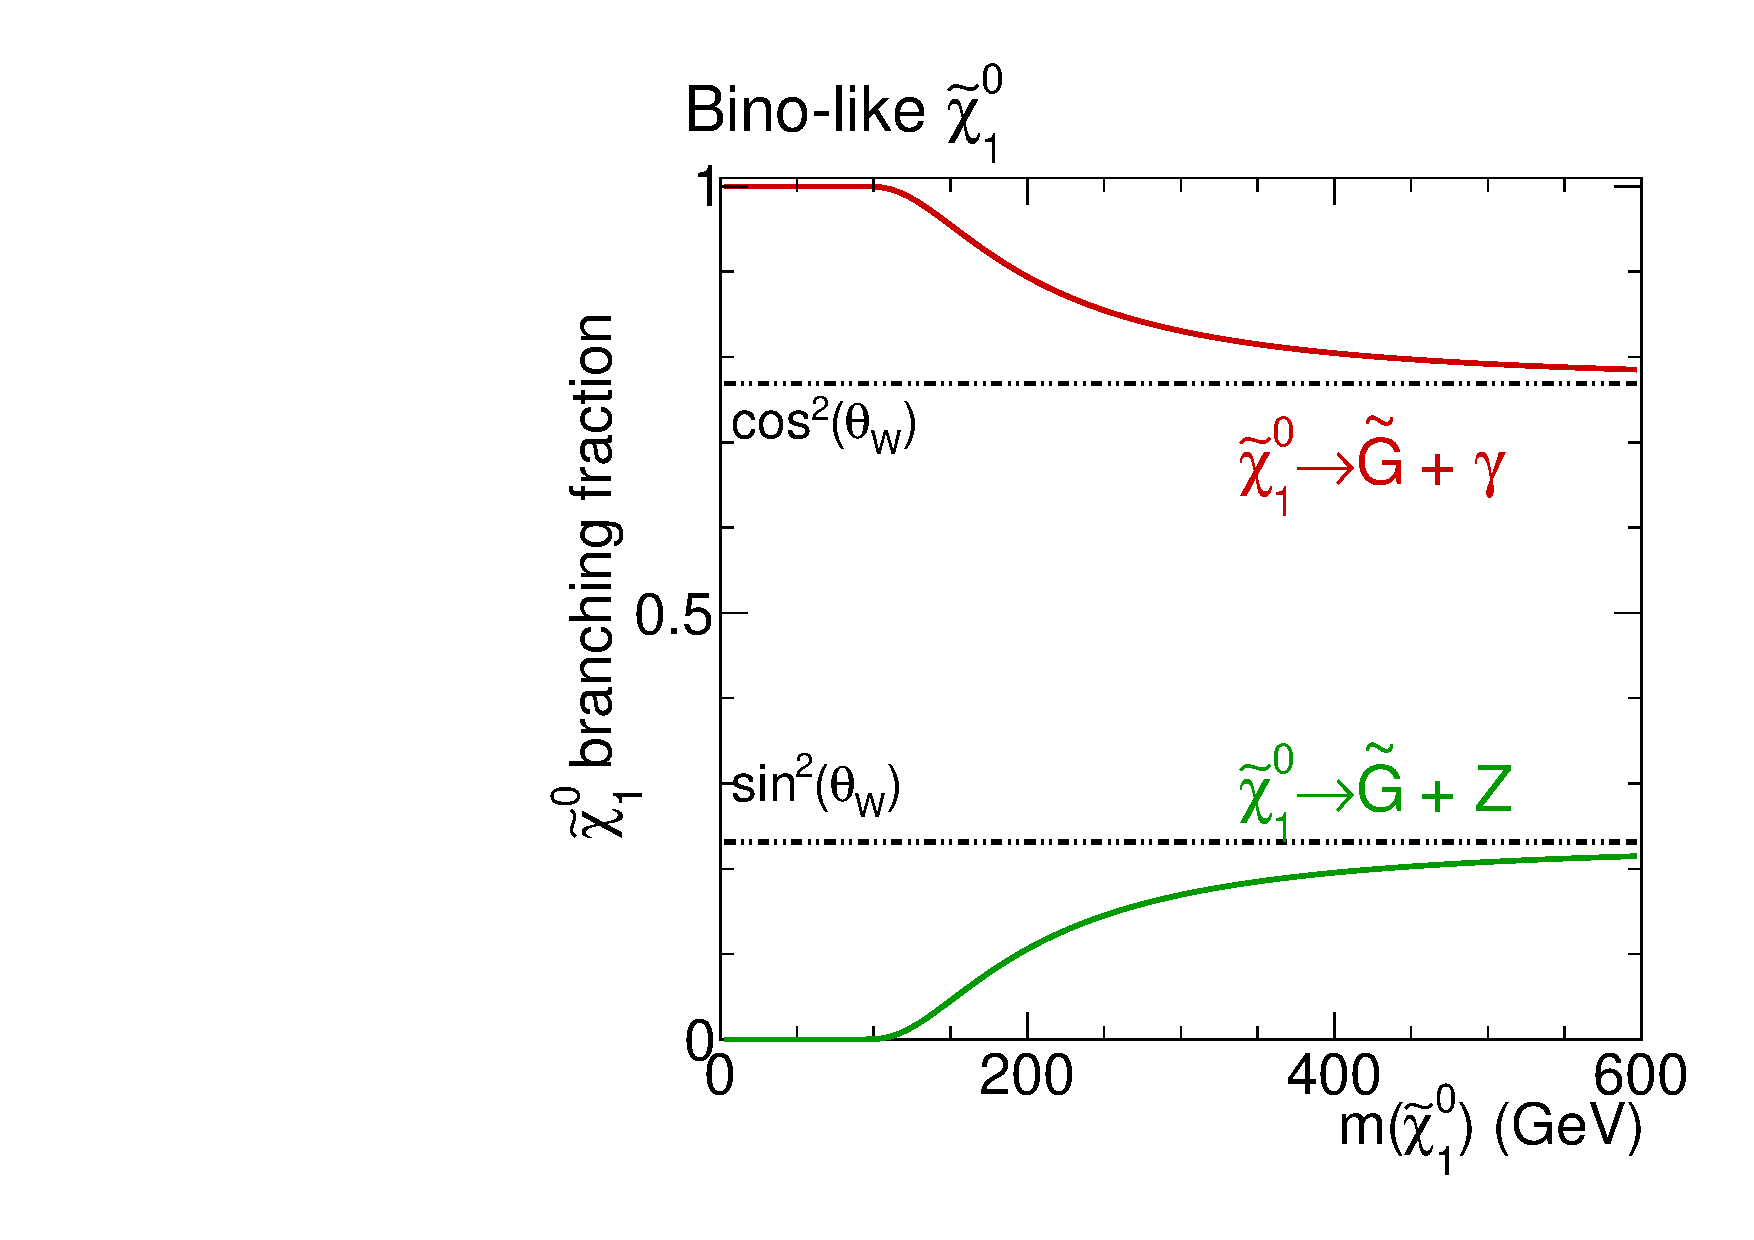
\includegraphics[width=\pairwidth]{figures/signal/binoBranching}
 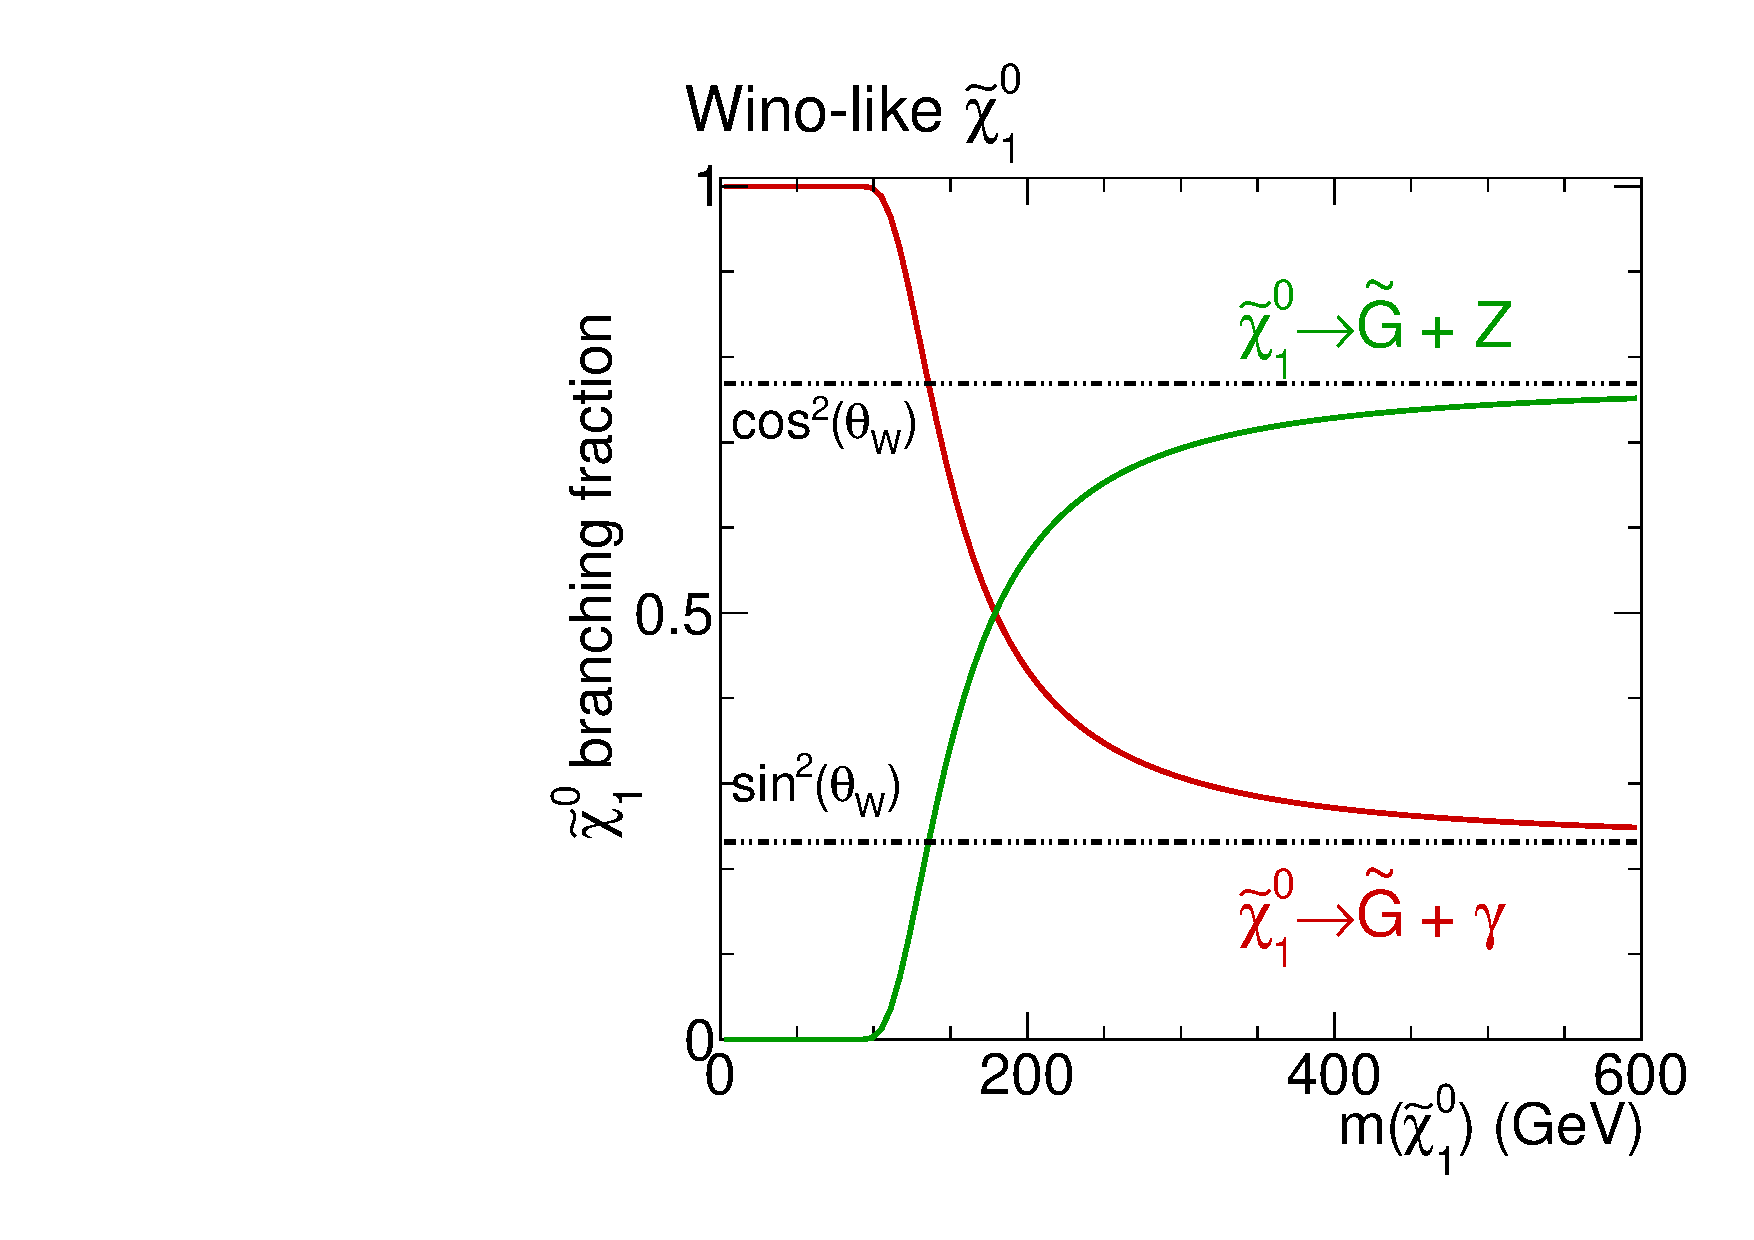
\includegraphics[width=\pairwidth]{figures/signal/winoBranching}%\\
 % 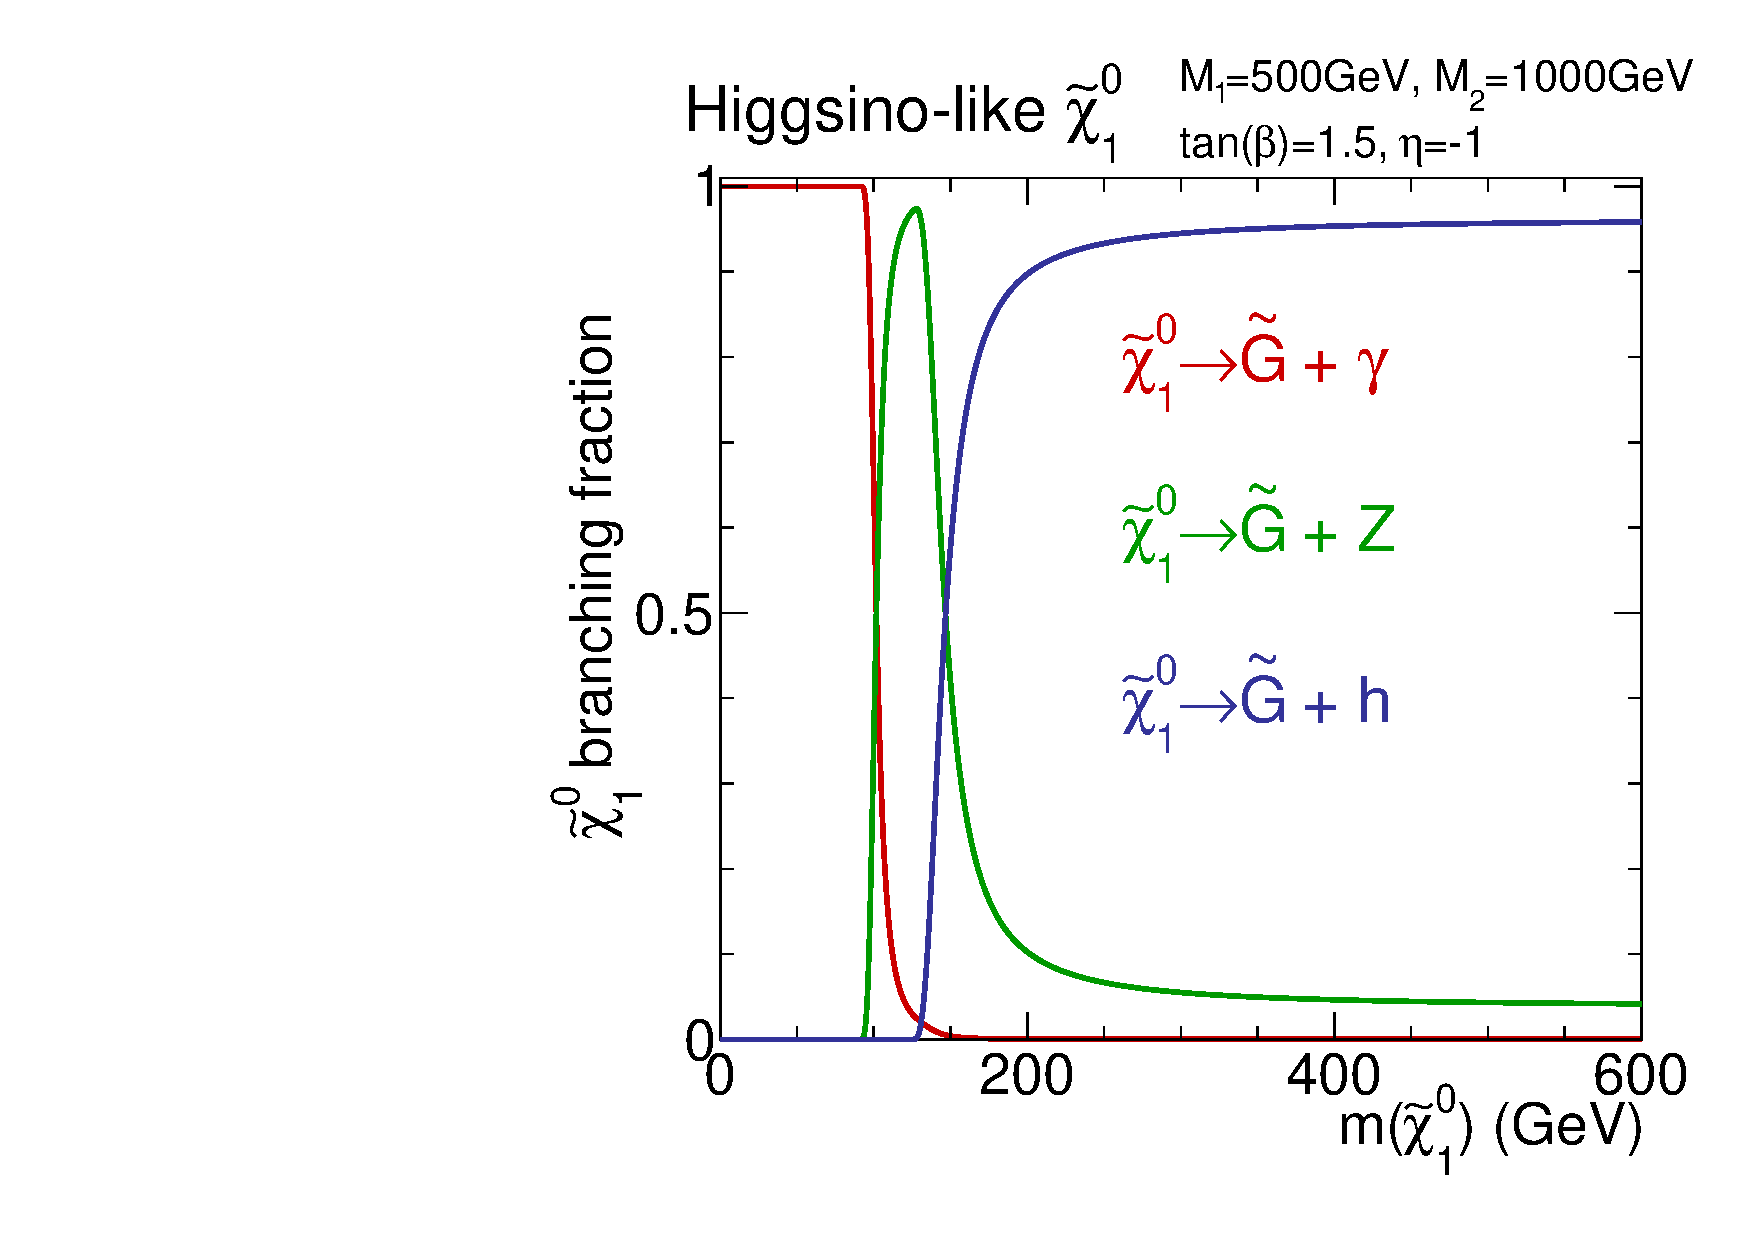
\includegraphics[width=\pairwidth]{figures/signal/higgsinoBranching1}
 % 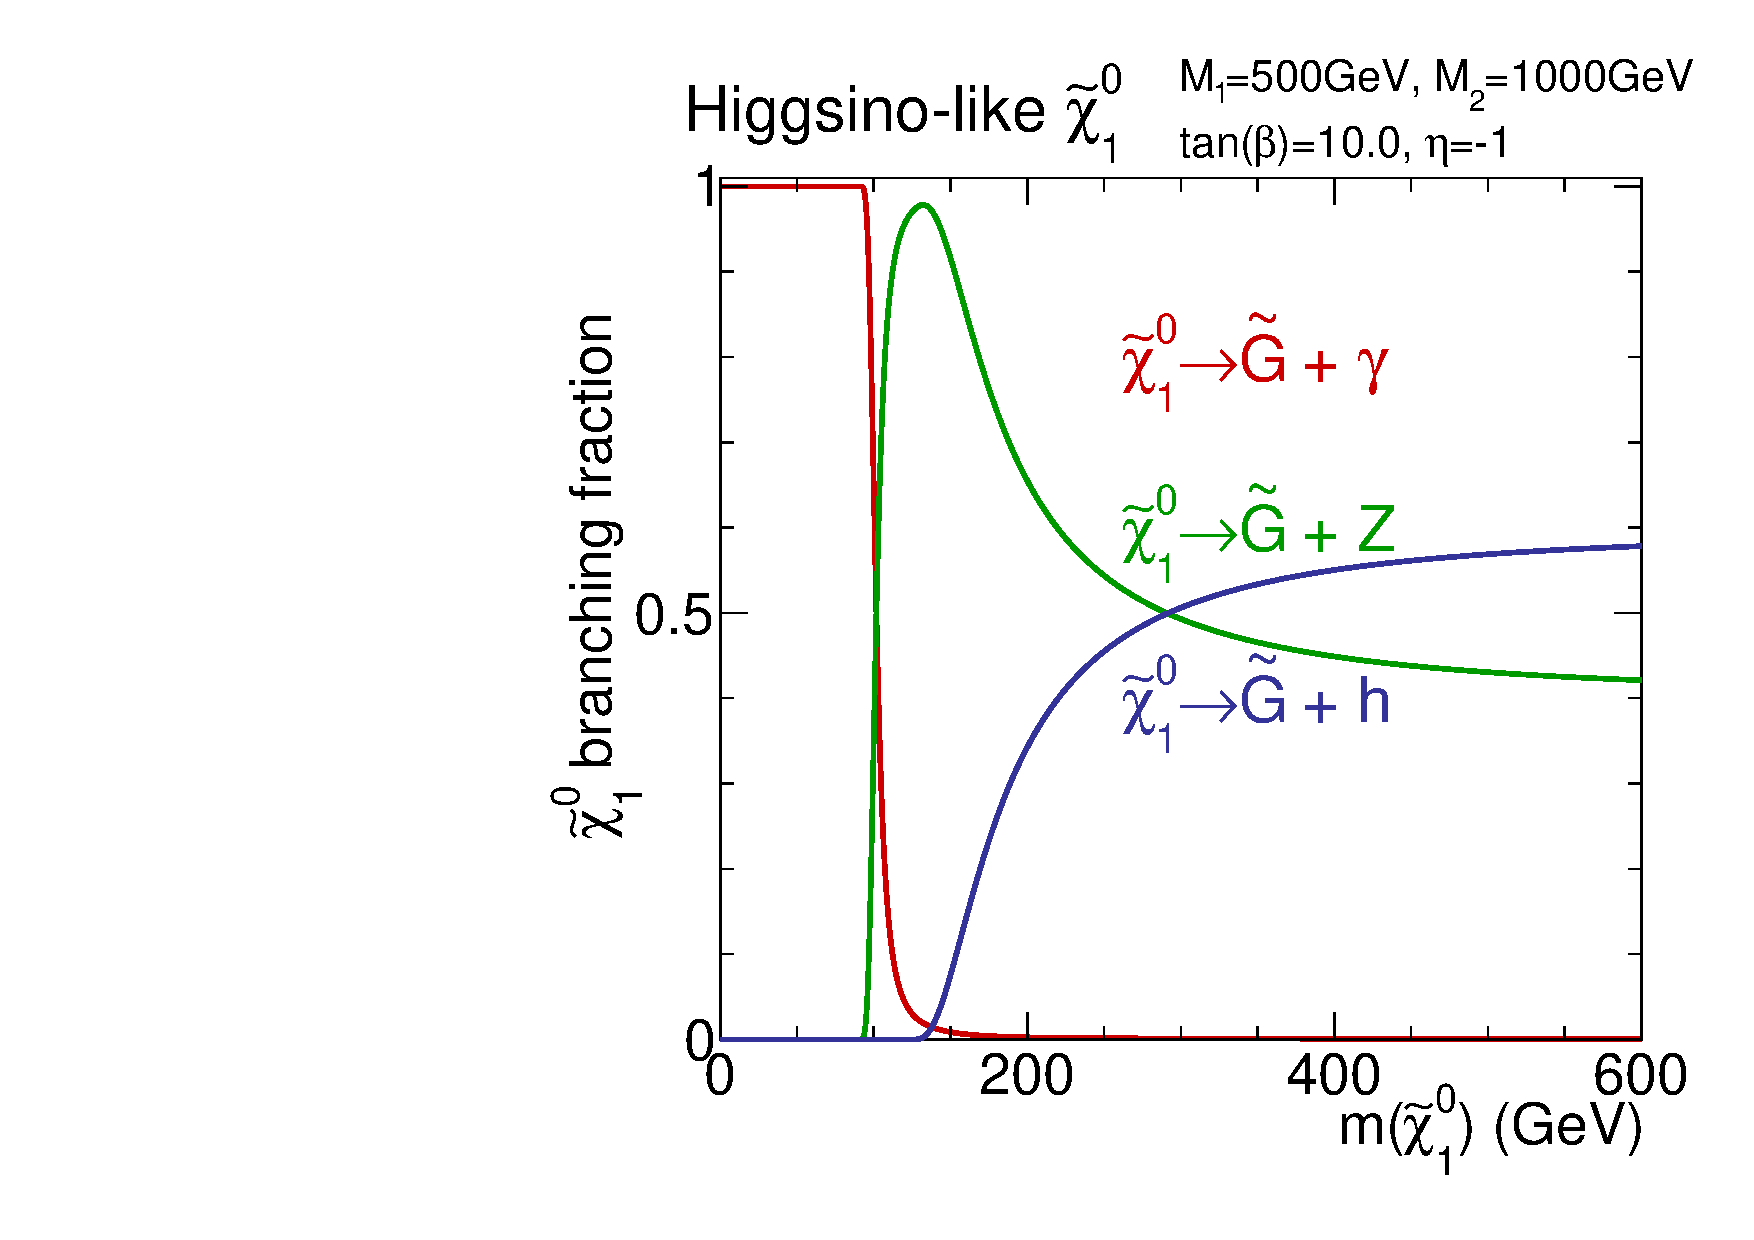
\includegraphics[width=\pairwidth]{figures/signal/higgsinoBranching2}
 % \caption{Branching fractions for pure bino (top left), wino (top right), and two higgsino-like (bottom) NLPS scenarios with different parameters. The parameter $\eta$ is defined as $\eta=sgn(\mu)$.}
 \caption{Branching fractions for pure bino (left) and wino (right) NLPS scenarios with different parameters~\cite{Kiesel}.}
 \label{fig:BRNLSP}
\end{figure}
Since the final state investigated in this analysis consists of a $\PZ$ boson and a photon, the search is sensitive in particular to bino- and wino-like NLSP scenarios.\\\\
One scenario used in the development of this search is a consistent GGM model, where the NLSP is the $\neutralinoOne$, and it is assumed to be bino-like. The heavier neutralino $\neutralinoTwo$ and the lightest chargino $\charginoOne$ are assumed to be wino-like. Therefore, the bino mass equals the mass of the lightest neutralino, while the $\PSGcpDo$ and the $\PSGczDt$ are mass degenerate and their mass equals the wino mass. Higgsinos are decoupled, \ie, set to very high masses. Squarks and gluinos are also decoupled in this scenario, allowing only electroweak production modes. For the most dominant process a diagram is shown in \refFig{fig:ewkSMS} right. The signal cross section depends only on the wino mass, since $\neutralinoTwo\PSGcpmDo$ and $\PSGcmpDo\PSGcpmDo$ production are by far the most dominant production channels. Branching fractions of the gauginos are given by the gaugino masses and their gauge eigenstates, and behave as shown in \refFig{fig:BRNLSP}. The mass of the neutralinos and the lightest chargino directly influence the transverse momenta in the final state. As can be seen in \refFig{fig:ewkSMS}, larger mass differences between the NLSP mass and the wino mass will lead to higher momenta of the produced bosons in the cascades. The mass of the NLSP is directly responsible for the momenta of the SM bosons and the gravitino in the final state, and therefore the missing transverse momentum in an event.
\begin{figure}[tbp]
 \centering
 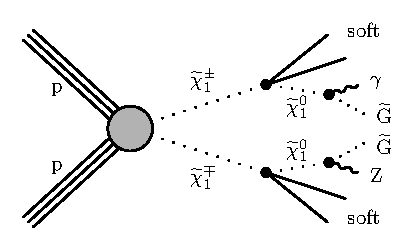
\includegraphics[width=0.49\textwidth]{figures/signal/TChiNG}
 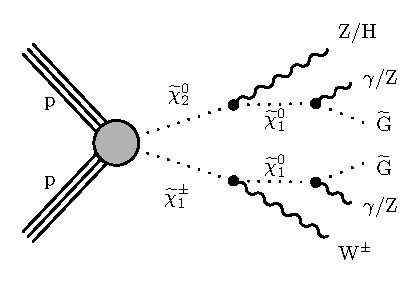
\includegraphics[width=0.49\textwidth]{figures/signal/gmsb}
 \caption{Diagram of the \texttt{TChiZG} scenario (left) with chargino pair production, where the charginos decay to neutralinos under soft emission of off-shell W bosons. Also, the chargino-neutralino production is possible. The most dominant production process with a wino-like $\PSGcpDo$ and $\PSGczDt$ of the full GMSB model (right).}
 \label{fig:ewkSMS}
\end{figure}
\\\\A very different approach in regard to the interpretation in full theoretical models are simplified models (SMS)\cite{SMS}. Here, only a limited particle content is assumed with simplified assumptions on the production and decay channels, providing a more model independent result by probing distinct final states. These results can be reinterpreted in various models~\cite{SMSReInt}. In this thesis two simplified models are considered, one with electroweak gaugino production, and the other one with a strong gaugino production channel.\\
The electroweak model is the \texttt{TChiZG} SMS, in which only neutralino-chargino and chargino-chargino production is assumed. The lightest chargino and lightest neutralino are assumed to have nearly the same mass, leading to soft emissions of off-shell W bosons in the decays of the charginos to the NLSP. The branching fractions of the lightest neutralino to a gravitino and a photon or a Z boson are fixed to $50\%$ each, \ie, $\mathcal{BR}(\PSGczDo\to\gamma\gravitino)=\mathcal{BR}(\PSGczDo\to\PZ\gravitino)=0.5$. A diagram for the process can be found in~\refFig{fig:ewkSMS} left. Squarks and gluinos are decoupled.\\
The strong model considered here is the \texttt{T5bbbbZG} SMS. A diagram is depicted in \refFig{fig:strongSMS}. In this model, gluino pair production is assumed, leading to decays to the NLSP under the emission of bottom quark pairs. The branching fractions for the $\PSGczDo$ to photons and Z bosons are again set to $50\%$ each.

\begin{figure}[tbp]
 \centering
 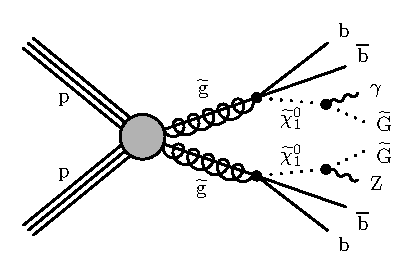
\includegraphics[width=0.49\textwidth]{figures/signal/T5bbbbZG-crop}
 \caption{The Feynman diagram for the \texttt{T5bbbbZG} scenario with pair production of gluinos in the hard process, decaying to neutralinos under the emission of b quarks.}
 \label{fig:strongSMS}
\end{figure}


\subsection{Status of SUSY searches at the Large Hadron Collider}
Searches for SUSY have been performed  at the LEP experiment~\cite{LEP}, the Tevatron collider~\cite{TEVATRON}, and using the LHC Run~I data~\cite{ChristianRunI}. Although some promising excesses with respect to the SM expectation have been observed for example in the opposite-sign dilepton channel~\cite{Edge}, no clear evidences for SUSY or other BSM theories have been confirmed. Currently SUSY is also constrained by precision measurements of the Higgs boson properties as mentioned above, and by measurements of rare decay processes, such as the $B_S^0\to\Pgmm\Pgmp$ decay observed by the CMS and LHCb collaborations~\cite{B0S}. In the SM, this decay is helicity suppressed, whereas in the MSSM or other extensions to the SM this decay may receive large enhancements.\\
Direct searches for SUSY in terms of SMS interpretations excluded gluino pair production up to gluino masses of around $2\TeV$~\cite{GluinoCMS}, squark pair production up to squark masses of roughly $1500\GeV$, and sbottom (stop) masses of approximately $1500\GeV$~\cite{sbottom} ($1200\GeV$~\cite{stop}), respectively. The production of electroweakinos (electroweak gauge bosinos) is excluded for chargino and neutralino masses up to around $1.1\TeV$~\cite{EWKinos}.
Regarding GMSB scenarios, the currently most stringent exclusion limits set by the CMS collaboration~\cite{CMS} are shown in \refFig{fig:GMSB_summary}.
\begin{figure}[tbp]
 \centering
 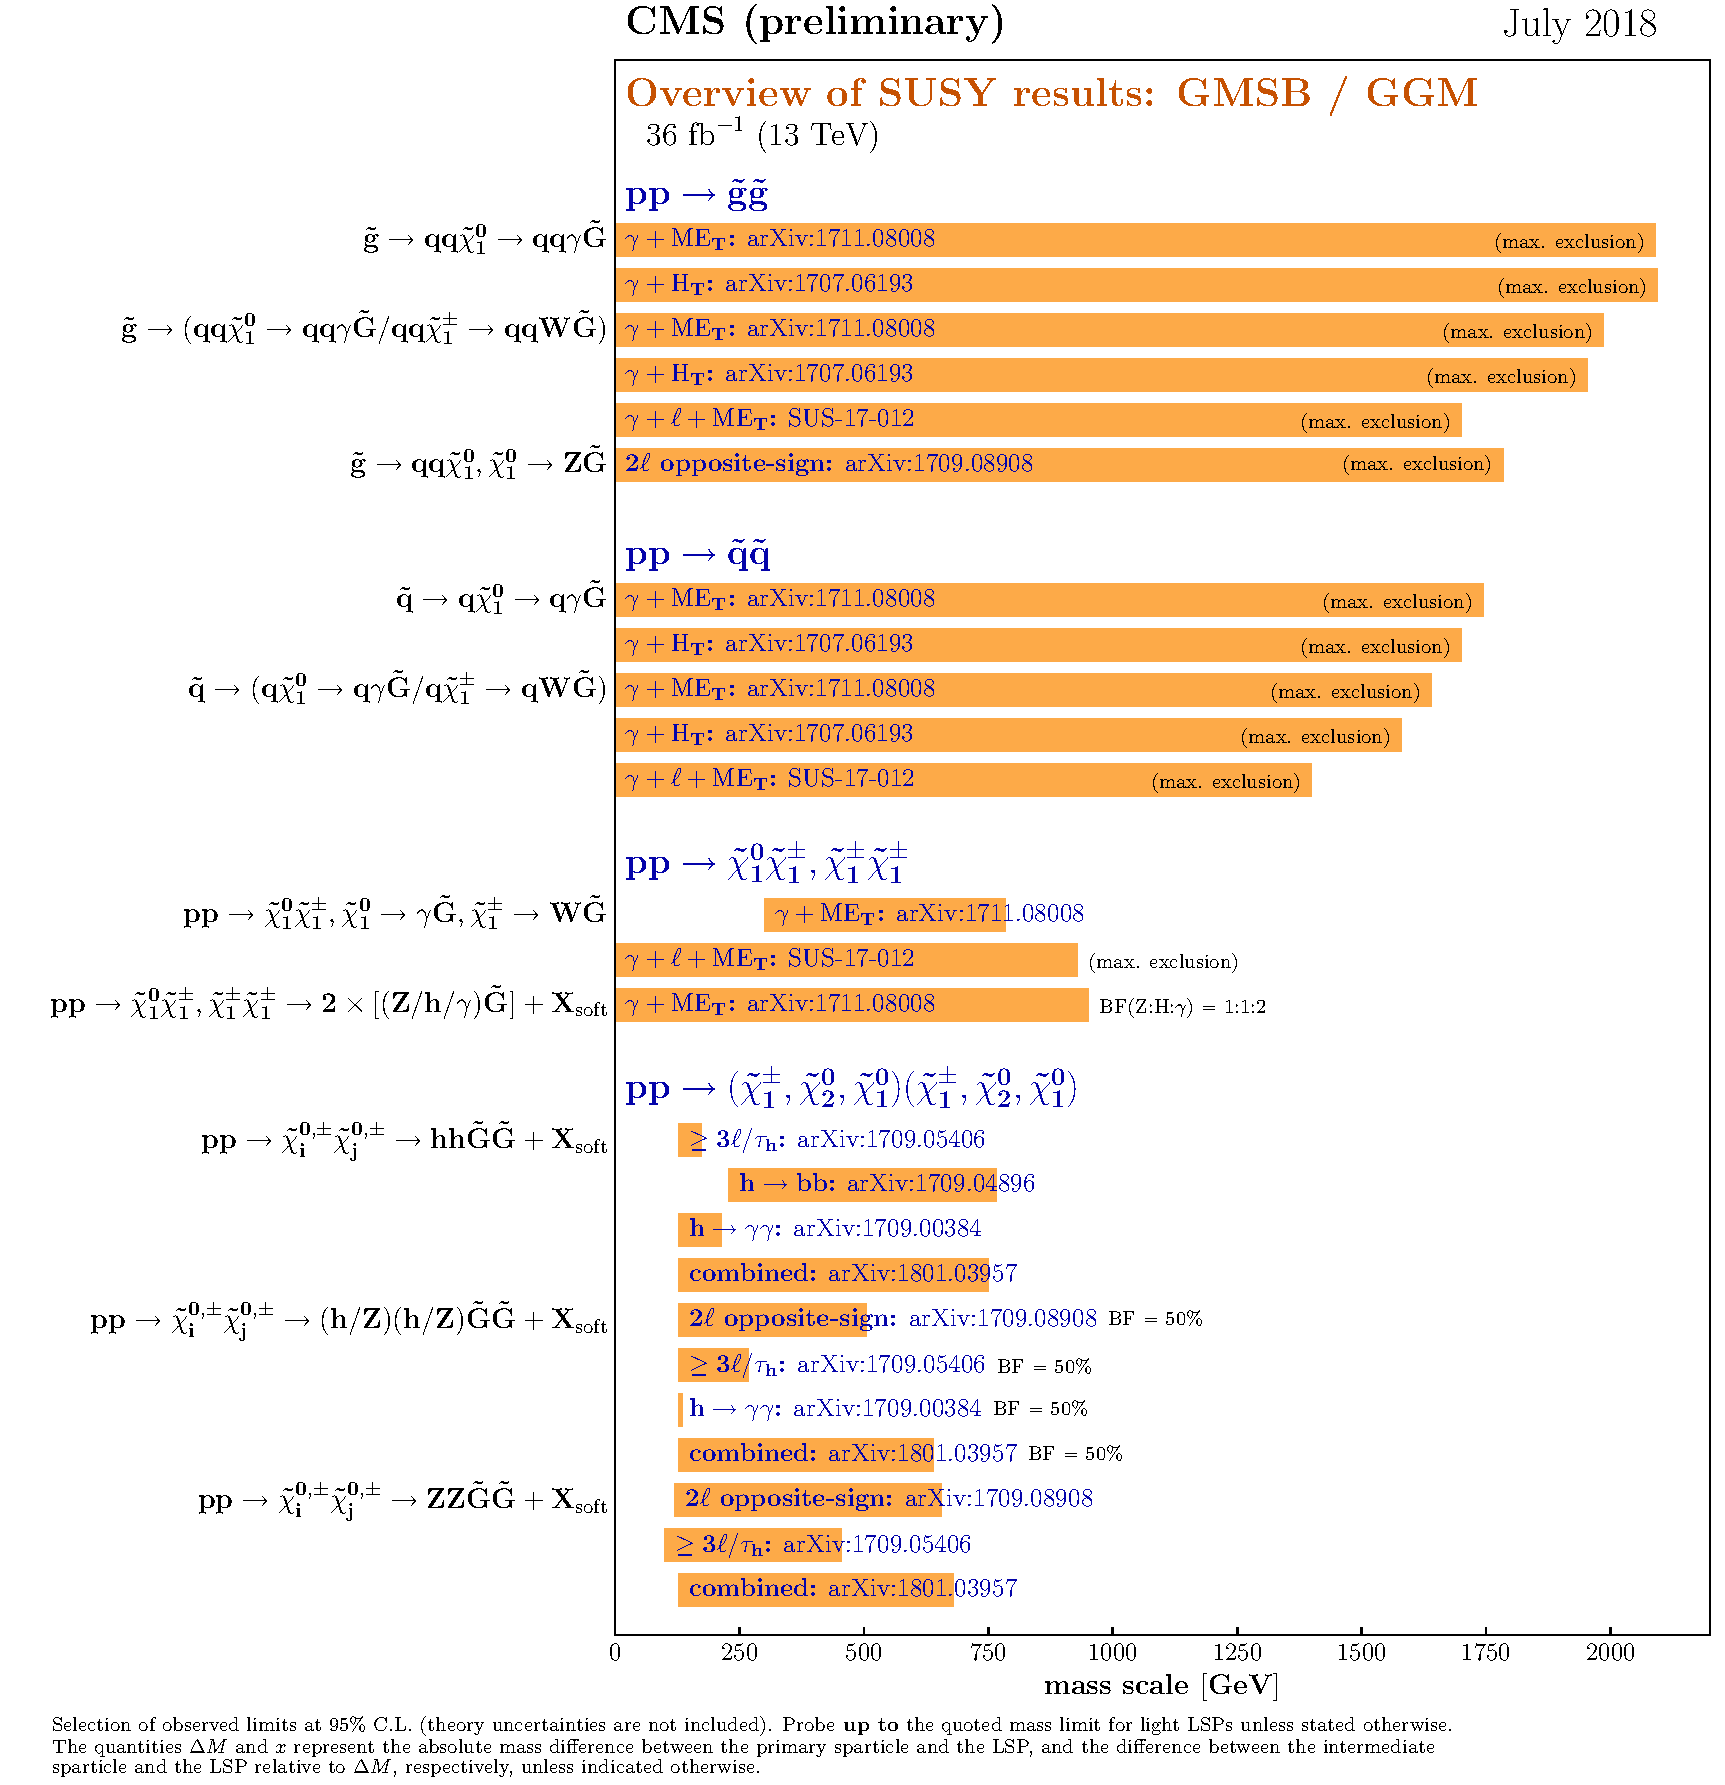
\includegraphics[width=0.99\textwidth]{figures/general/barplot_GMSB}
 \caption{Mass exclusion limits for simplified models in the context of GMSB of the CMS collaboration~\cite{SUSSummaryPlot}.}
 \label{fig:GMSB_summary}
\end{figure}
The presented results are based on the proton-proton collision data recorded with the CMS detector in 2016, corresponding to an integrated luminosity of $36\fbinv$ with a center-of-mass energy of $\sqrt{s}=13\TeV$. Searches similar to the one presented in this thesis exclude electroweakino production scenarios up to roughly $980\GeV$, when final states tagged with a high-energy photon and large missing transverse momentum are analyzed~\cite{PhotonMet}. Searches targeting the single lepton plus photon final state~\cite{PhotonLepton} have set lower limits. Strong exclusions for gluino and squark pair production scenarios are set by searches targeting events with large hadronic activity and photons~\cite{PhotonHT} and searches investigating events with photons together with high b-jet multiplicity~\cite{PhotonBJet} over the whole parameter space. They set limits up to approximately $2.2\TeV$ for gluino masses and $1.8\TeV$ for squark masses.\\
Despite the high exclusion limits set by CMS and ATLAS analyses~\cite{AtlasGMSB1,AtlasGMSB2,AtlasGMSB3} in comparable ways, large regions of phase space remain unexplored. But since there are many different SUSY models, and the phenomenology of SUSY is very rich, including scenarios with R-parity violation, compressed mass spectra, long-lived particles and displaced vertices, all described in different breaking scenarios, many studies and searches are yet to be performed. Nevertheless, although the sparticle masses are not predicted by theory, natural SUSY scenarios without great fine tuning should lead to sparticle masses in the order of $\mathcal{O}(\TeV)$, which are accessible at the LHC~\cite{SUSYNaturalStatus}.
